\documentclass[english]{article}
%\usepackage[a4paper]{geometry} % senza abbiamo problemi con le tabelle
\usepackage[T1]{fontenc}
\usepackage[utf8]{inputenc}
\usepackage{babel}
\usepackage[unicode=true,pdfusetitle,
 bookmarks=true,bookmarksnumbered=false,bookmarksopen=false,
 breaklinks=true,pdfborder={0 0 1},backref=false,colorlinks=false]
 {hyperref}
\usepackage{tabularx}
\usepackage{graphicx}
\graphicspath{{images/}{Mockups/}}
\usepackage{svg}
\renewcommand{\arraystretch}{1.4}

\begin{document}

\title{Politecnico di Milano\\
 A.A. 2016–2017 \\
Software Engineering 2: “PowerEnJoy” \\
\emph{Requirements Analysis and Specification Document}}

\author{Pietro Ferretti, Nicole Gervasoni, Danilo Labanca}

\maketitle
\newpage{}

\tableofcontents{}

\newpage{}

\section{Introduction}

\subsection{Purpose}

\paragraph{}
The purpose of this document is to provide a detailed description and specification of a digital management system for PowerEnJoy, an electric car sharing service. This document will
illustrate functional and non-functional requirements of the software to-be, outlining costraints, showing potential user interfaces for the software, and explaining the domain assumptions made. Additionally, at the end of the document we will present an Alloy model to further specificate the world and environment our system will have to manage.

\paragraph{}
This document is first and foremost a description of the project for all interested stakeholders and a reference for future development, but can also be used as a basis for legally binding agreements.


\subsection{Scope}

\paragraph{}
The aim of this project is to specify in detail a new digital management software for PowerEnJoy, a car-sharing service that employs electric cars only.

\paragraph{}
Users must be able to register to PowerEnJoy providing their personal data, driving license and payment information.
After registering, users should be able to look for available cars near them or to a specific location. If they find a car that matches their needs, they can reserve the car up to one hour before using it. After approaching a reserved car users should have a way to unlock the car and enter it.
While using a car users are charged a certain amount of money depending on distance traveled and time elapsed; while driving the car a display will inform the user of the amount of money they will have to pay at the end of the ride.
The system stops charging the user after the car is parked in a safe area.
Furthermore the system incentivizes virtuous behaviours by offering several discounts if certain conditions are met (e.g. charging a car at a power grid station).

\paragraph{}
To accomplish these goals we need to bridge the gap between the world (cars and passengers) and our system (servers, databases, etc.).
The users will be able to access the system functionalities through a web and a mobile application, and a dedicated touchscreen installed in every car.
A central system will manage the cars and the reservations, and will communicate with the cars through the Internet. The system will follow the cars’ movements thanks to the GPS tracker installed in every car. Furthermore all cars will be equipped with a great variety of sensors to check the cars’ status at any time.


\subsection{Definitions, Acronyms, Abbreviations}

\subsubsection{Definitions}

\begin{itemize}
\item{\textit{Guest}: a person that is not registered to the system.}
\item{\textit{User}: a person that is registered to the system. Users can log in to the system with their email or username and their password. Their first name, last name, date of birth, driving license ID are stored in the database.}
\item{\textit{Safe area}: a location where the user can park and leave the car. Users can end their ride and park temporarily only in these locations. The set of safe areas are predefined by the system.}
\item{\textit{Power grid station}: a place where cars can be parked and plugged in. While a car is plugged in a power grid station its battery will be recharged. Power grid stations are by definition safe areas.}
\item{\textit{Available car}: a car that is currently not being used by any user, and has not been reserved either. Available cars are in good conditions (not dirty nor damaged) and don’t have dead batteries.}
\item{\textit{Reservation}:
	\begin{itemize}
		\item{the operation of making a car reserved for a user, i.e. giving permission to unlock and use the car only for that user, forbidding reservations by other users.}
		\item{the time period between the moment a reservation is requested and the moment the user unlocks the car, or the reservation is canceled.}
	\end{itemize}
}
\item{\textit{Ride}: the time period from the moment a reserved car is unlocked to the moment the user notifies that he wants to stop using the car and closes all the doors. A ride doesn’t stop when a car is temporarily parked, but continues until the user chooses to leave the car definitely.}
\item{\textit{Possession}: users that have reserved and unlocked a car are said to have possession of the car. While a user has possession of a car they are the only person that can drive it, lock or unlock it, and no other person can take possession of it until the user frees it. Users lose possession of a car when their ride ends.}
\item{\textit{Temporary parking}: the act of parking a car in a safe area and, after notifying the system, locking it and leaving it for a finite amount of time. The user that does this retains the right to use the car and can unlock it later to use it again.}
\item{\textit{Bill}: a record of the money owed by the user at the end of a ride.}
\item{\textit{Outstanding bill}: a bill that hasn’t been paid yet. }
\item{\textit{Suspended user}: a user that cannot reserve or use cars. Usually users are suspended because they have outstanding bills.}
\item{\textit{Payment method}: a way to transfer money from the user to the system. Our system will only accept credit cards and online accounts like Paypal.}
\item{\textit{Payment API}: an interface to carry out money transactions, offered by the external provider associated to the payment method used (e.g. a bank).}
\end{itemize}

\subsubsection{Acronyms}
\begin{itemize}
\item{\textbf{RASD}: Requirements Analysis and Specification Document}
\item{\textbf{DB}: Database}
\item{\textbf{CVV}: Card Verification Value}
\item{\textbf{DOB}: Date of birth}
\item{\textbf{PGS}: Power Grid Station}
\item{\textbf{GPS}: Global Positioning System}
\end{itemize}

\subsubsection{Abbreviations}
\begin{itemize}
\item{\textbf{[Gx]}: Goal}
\item{\textbf{[RE.x]}: Functional Requirement}
\item{\textbf{[UC.x]}: Use Case}
\end{itemize}

\subsection{Reference Documents}

\begin{itemize}
	\item{ISO/IEC/IEEE Std. 29148:2011, “Systems and software engineering -- Life cycle processes -- Requirements engineering”}
	\item{Specification document: “Assignments AA 2016-2017.pdf”}
\end{itemize}

\subsection{Document Overview}

\newpage{}

\section{Overall Description}

\subsection{Product Perspective}

\subsection{Product Functions}

The PowerEnJoy application will offer many different functionalities; specifically, the goals we want to accomplish are the following:
\begin{description}
	\item[{[G1]}]{Guests must be able to register as users by choosing a username and providing their personal data, driving license and payment information. They will receive a password at the email address they specified.}
	\item[{[G2]}]{Users must be able to login with the username/email inserted and the password received on registration.}
	\item[{[G3a]}]{Users must be able to find the location and battery charge of all the available cars within a certain distance from their current location.}
	\item[{[G3b]}]{Users must be able to find the location and battery charge of all available cars around a specified location.}
	\item[{[G4]}]{Users must be able to reserve a car for up to one hour before they pick it up. If they don't take the car before the time expires they are charged a fixed fee of 1 EUR.}
	\item[{[G5]}]{Users must be able to cancel a reservation if they decide to not actually use the car.}
	\item[{[G6]}]{A user that reaches a car reserved by them must have a way to tell the system they’re nearby, so that the system unlocks the car and the user may enter.}
	\item[{[G7]}]{The system must charge the user who reserved the car from the moment the engine is ignited after unlocking it. The amount charged depends on the distance traveled and time elapsed.}
	\item[{[G8]}]{The system must allow the user to see the amount they’re being charged through a screen on the car.}
	\item[{[G9]}]{The system must stop charging the user as soon as the car is parked in a safe area and the user exits the car notifying the system that they ended their ride.}
	\item[{[G10]}]{Users must be able to leave a car without losing the reservation by informing the system that they’re only temporarily parking; in this case the system continues on charging the user. The user should be able to end the ride without coming back to the car if they so choose.}
	\item[{[G11]}]{The system must lock the car automatically after the user exits the car.}
	\item[{[G12]}]{The system must provide a money saving option to the user, proposing a suitable power grid station near the user’s final destination. The user will get a discount if they park the car there and plug it in the power grid.}
	\item[{[G13]}]{The stations proposed by the system with the money saving option must be chosen in a way that ensures a uniform distribution of cars in the city.}
	\item[{[G14]}]{The system must apply a discount of 10\% on the last ride if the user took at least two other passengers onto the car.}
	\item[{[G15]}]{The system must apply a discount of 20\% on the last ride if the car is left with more than 50\% of remaining battery charge.}
	\item[{[G16]}]{The system must apply a discount of 30\% on the last ride if the car is left at special parking areas where they can be recharged, and the user takes care of plugging the car into the power grid.}
	\item[{[G17]}]{The system must charge 30\% more if the car is left at more than 3 km from the nearest power grid station or with less than 20\% remaining battery charge.}
	\item[{[G18]}]{Users with outstanding bills cannot have access to the cars and reservations until the bills are paid.}
	\item[{[G19]}]{Users with outstanding bills should have a way to pay them.}
	\item[{[G20]}]{Available cars should actually be available to the user and in good conditions (i.e. not dirty, damaged, and/or with low battery)}
\end{description}

\subsection{User Characteristics}

\subsection{Constraints}\label{constraints}

To provide all the functionalities specified in this document, every car must have:
\begin{itemize}
	\item{a reliable GPS tracker}
	\item{a mobile Internet connection (for example a 3G or 4G connection)}
	\item{sensors to collect data from the engine and the battery}
	\item{an electronic switch to lock and unlock the doors}
	\item{a weight sensor on each seat}
	\item{a touchscreen to offer a dedicated interface to users}
	\item{an internal system to control these components and communicate\\ with the central system}
	\item{a unique qr code printed on the outside of the car}
\end{itemize}

\paragraph{}
\emph{and we need a GPS navigator on the car to find power grid stations}

\paragraph{}
The web application needs an Internet connection to work, for example to connect to the database and find available cars.

\paragraph{}
The mobile application will need at least an Internet connection to receive data from and communicate with the central system. Access to the device’s location is not mandatory, but is needed to provide the “find available cars near me” functionality.

\subsection{Assumptions and Dependencies}

\emph{See section \ref{constraints} for hardware assumptions.}


The system has a predefined list of all the safe areas and their locations.

The system has a predefined list of all the power grid stations and their locations.

The system knows how many plugs are present in each station and how many of them are free in a given moment.


The car’s data connection is always working and stable

The car’s GPS signal is always available and precise


After unlocking a car users turn on the engine shortly after (i.e. the user doesn't stand in the car idly for long periods of time). We suppose that the user wants to get to their destination as soon as possible.


When the user has ended the reservation or chosen to temporarily park from the car’s screen, we assume that the users and all the passengers have exited the car before the last door is closed.


When the weight measured by a seat weight sensor exceeds a certain threshold, it means that a person is present on that seat (and not an object).


Stolen cars are handled by someone else (police, lawyers)


A phone line is available in case of car accidents or damage to the car.

-> insurance, assistance, fines


An external agency is entrusted with the task of charging cars with low or dead batteries.


An external agency is entrusted with the task of regularly cleaning the inside and outside of cars.

Users always report dirty or damaged cars

Users don't let the cars run out of battery before parking in a safe area. (Otherwise they call a phone line and pay a fee)

\newpage

\section{Specific Requirements}

\subsection{External Interface Requirements}

\subsubsection{User Interfaces}
web
\begin{figure}
	\centering
	\makebox[\textwidth][c]{	
		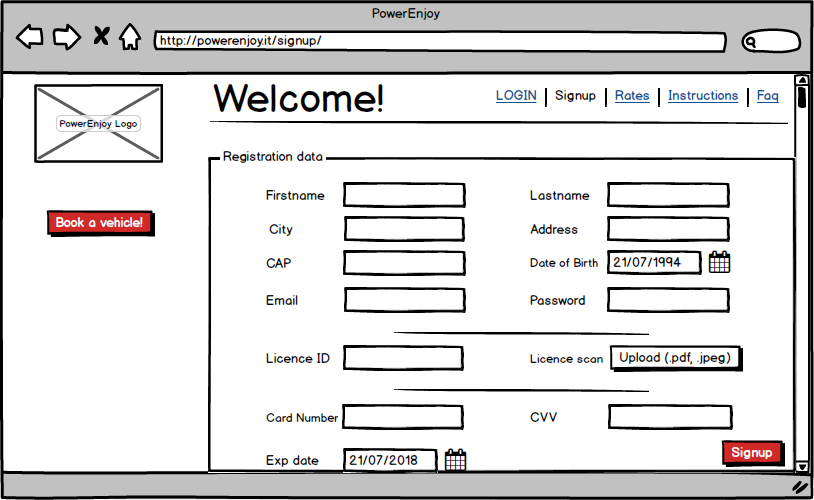
\includegraphics[width=\textwidth]{web/Signup.png}
	}
	\caption{*signup*}
\end{figure}
\begin{figure}
	\centering
	\makebox[\textwidth][c]{	
		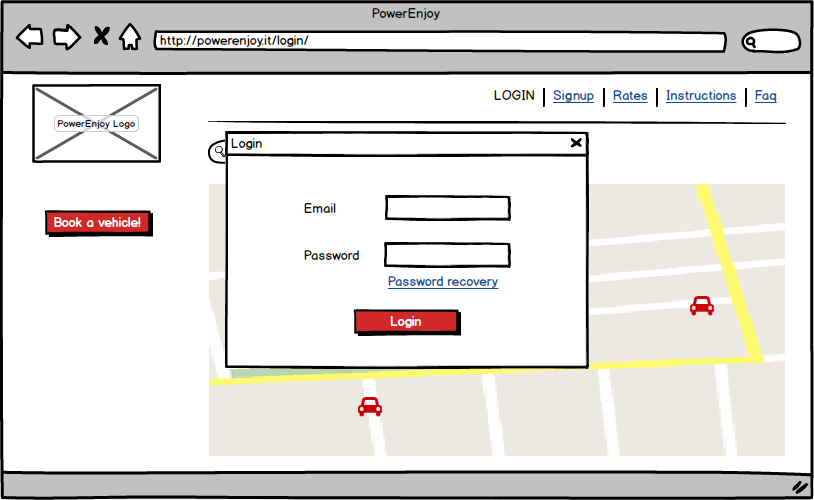
\includegraphics[width=\textwidth]{web/Login.png}
	}
	\caption{*login*}
\end{figure}
\begin{figure}
	\centering
	\makebox[\textwidth][c]{	
		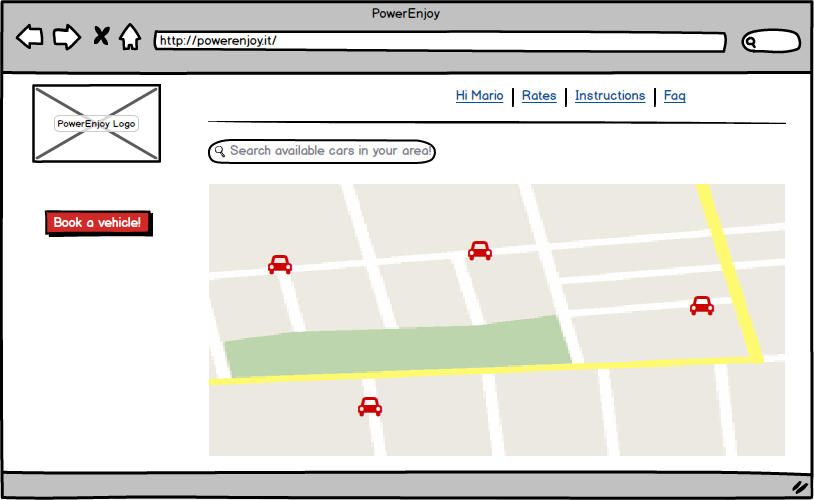
\includegraphics[width=\textwidth]{web/HomepageLogged.png}
	}
	\caption{*homepage*}
\end{figure}
	
mobile
\begin{figure}[h]
	\centering
	\makebox[\textwidth][c]{	
		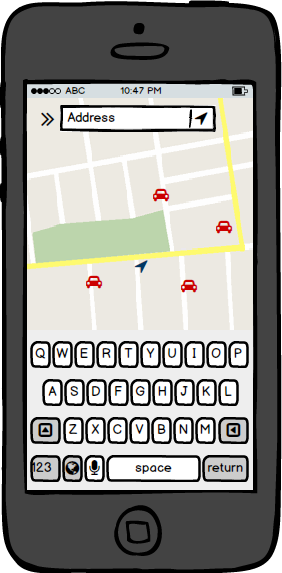
\includegraphics[width=\textwidth]{mobile/localization.png}
	}
	\caption{*mappa*}
\end{figure}
\begin{figure}
	\centering
	\makebox[\textwidth][c]{	
		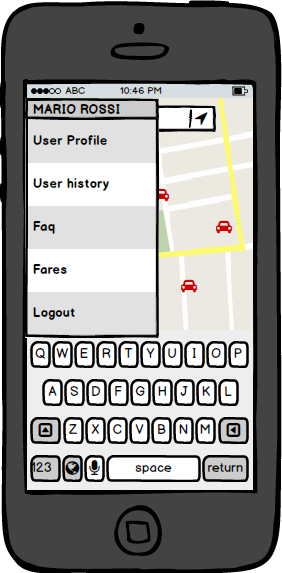
\includegraphics[width=\textwidth]{mobile/MenuSX.png}
	}
	\caption{*menu*}
\end{figure}
\begin{figure}
	\centering
	\makebox[\textwidth][c]{	
		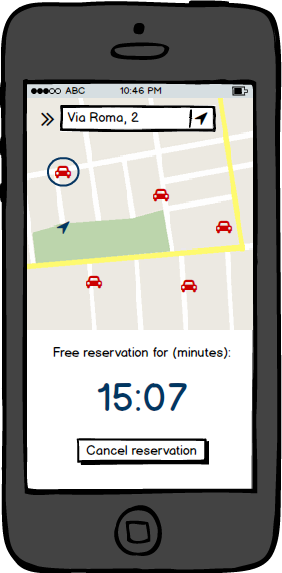
\includegraphics[width=\textwidth]{mobile/FreeReservation.png}
	}
	\caption{*reservation*}
\end{figure}
\begin{figure}
	\centering
	\makebox[\textwidth][c]{	
		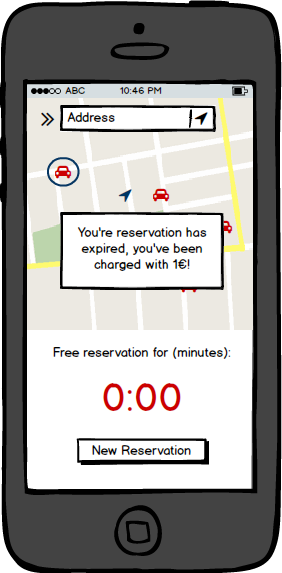
\includegraphics[width=\textwidth]{mobile/FreeReservationEnded.png}
	}
	\caption{*reservation expired*}
\end{figure}
\begin{figure}
	\centering
	\makebox[\textwidth][c]{	
		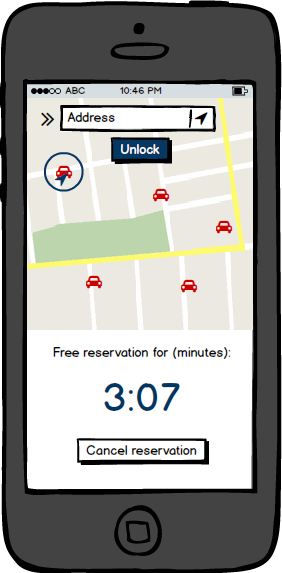
\includegraphics[width=\textwidth]{mobile/Unlock.png}
	}
	\caption{*unlocking*}
\end{figure}

car's display
\begin{figure}
	\centering
	\makebox[\textwidth][c]{	
		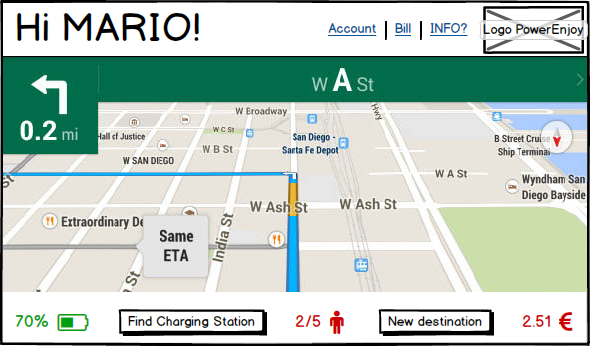
\includegraphics[width=\textwidth]{car/car.png}
	}
	\caption{*car's display*}
\end{figure}
\subsubsection{Hardware Interfaces}

\subsubsection{Software Interfaces (API)}

\subsubsection{Communication Interfaces}

\newpage
\subsection{Functional Requirements}

\subsubsection{Requirements}


\begin{description}

\item[{[G1]}]{Guests must be able to register as a user by choosing a username and providing their personal data, driving license and payment information. They will receive a password at the email address they specified.

\begin{itemize}
\item{[RE.1.1] The system must offer an interface (e.g. a form on a web page or on the mobile application) where the user can enter and submit the data needed for registration:
a username of their choice, their personal data (first name, last name, date of birth), a driving license ID or a photo of one, and a payment method.}
\item{[RE.1.2] The system must verify that the data provided by a user on registration is valid.}
\item{[RE.1.3] When a user registers the system must randomly generate a safe password and associate it to the user’s account.}
\item{[RE.1.4] After a user is registered the system must send the generated password to the user via email at the email address they provided.}
\end{itemize}
}

\item[{[G2]}]{Users must be able to log in with the username/email they submitted on registration and the password they received.
\begin{itemize}
	\item{[RE.2.1] The system must offer an interface (e.g. a form on a web page or on the mobile application) where the user can enter and submit their credentials (username/email and password) to log in.}
	\item{[RE.2.2] The system must compare the credentials submitted by the user with the ones saved in the database.}
	\item{[RE.2.3] If the credentials submitted on login are valid, the system authenticates the user and allows them to use the available functionalities.}
	\item{[RE.2.4] If the credentials submitted on login are not valid, the system denies access to the user and notifies them of the error.}
\end{itemize}
}

\item[{[G3a]}]{Users must be able to find the location and battery charge of all the available cars within a certain distance from their current location.
\begin{itemize}
	\item{[RE.3a.1] The system must offer an interface where the user can activate the option to look for nearby available cars if the user’s location is available (e.g. thanks to a GPS receiver).}
	\item{[RE.3a.2] When the user activates the option to find nearby available cars, the system must get the user's location and look in the database for every available car near them.}
	\item{[RE.3a.3] The system must show the results of the search for nearby available cars on a suitable interface (e.g. a map).}
\end{itemize}
}

\item[{[G3b]}]{Users must be able to find the location and battery charge of all available cars around a specified location.
\begin{itemize}
	\item{[RE.3b.1] The system must offer an interface where the user can submit an address and search for available cars near that location.}
	\item{[RE.3b.2] When the user starts a search for available cars near a certain address, the system must look in the database for every available car close to the address provided by the user.}
	\item{[RE.3b.3] The system must show the results of the search for available cars on a suitable interface (e.g. a map).}
\end{itemize}
}

\item[{[G4]}]{Users must be able to reserve a car for up to one hour before they pick it up.
\begin{itemize}
	\item{[RE.4.1] The system must offer an interface that shows to the user the cars available for reservation (e.g. the search results specified in RE.3a.3) and allow the user to select a car.}
	\item{[RE.4.2] When a user selects a car for reservation the system must mark the car as reserved by that user.}
	\item{[RE.4.3] If the car has not been unlocked for an hour after reservation, the system must mark the car as available and charge the user a fixed amount (1 EUR).}
\end{itemize}
}

\item[{[G5]}]{Users must be able to cancel a reservation if they decide to not actually use the car.}

\item[{[G6]}]{A user that reaches a car reserved by them must have a way to tell the system they’re nearby, so that the system unlocks the car and the user may enter.
\begin{itemize}
	\item{[RE.6.1] The system must offer an interface to unlock the car, with their position or the car's qr code.}
	\item{[RE.6.2] If the user is within a certain distance from the car, their device location is available and they choose from the interface to unlock the car with the position, the system must unlock the car.}
	\item{[RE.6.3] If the user chooses from the interface to unlock the car with the qr code and the user takes a clear picture of the qr code of the right car, the system must unlock the car.}
\end{itemize}
}

\item[{[G7]}]{The system must charge the user who reserved the car from the moment the engine is ignited after unlocking it. The amount charged depends on the distance traveled and time elapsed.
\begin{itemize}
	\item{[RE.7.1] The system must keep track until the end of the reservation of the amount the user has to pay.}
	\item{[RE.7.2] The system starts to charge the user the moment the reserved car’s engine is ignited after unlocking the car.}
	\item{[RE.7.3] The amount charged by the system depends on the time elapsed and the distance traveled by the user, following specific rules.}
\end{itemize}
}

\item[{[G8]}]{The system must allow the user to see the amount they’re being charged through a screen on the car.
\begin{itemize}
	\item{[RE.7.1] The system must keep track until the end of the reservation of the amount the user has to pay.}
	\item{[RE.8.1] After the system has started keeping track of the amount that the user has to pay, the system must show it in a clear way on the car screen while the car is in use and the reservation hasn’t ended.}
\end{itemize}
}

\item[{[G9]}]{The system must stop charging the user as soon as the car is parked in a safe area and the user exits the car after ending the reservation.
\begin{itemize}
	\item{[RE.7.1] The system must keep track until the end of the reservation of the amount the user has to pay.}
	\item{[RE.9.1] The moment a car is parked in a safe area, the system must ask through an interface on the car screen if the user wants to end the reservation or just park temporarily.}
	\item{[RE.9.2] If a reserved car has been parked in a safe area and the user has chosen to end the reservation, then after the user has closed the doors the system must carry out the transaction for the amount that the system calculated, with the method of payment specified by the user on registration.}
\end{itemize}
}

\item[{[G10]}]{Users must be able to leave a car in a safe area without losing the reservation by informing the system that they’re only temporarily parking; in this case the system keeps charging the user.
\begin{itemize}
	\item{[RE.7.1] The system must keep track until the end of the reservation of the amount the user has to pay.}
	\item{[RE.9.1] The moment a car is parked in a safe area, the system must ask through an interface on the car screen if the user wants to end the reservation or just park temporarily.}
	\item{[RE.10.1] When a car is temporarily parked and locked, the system keeps on charging the user but with different rules than those used in RE.7.3, this time depending only on time elapsed while parked.}
	\item{[RE.10.2] After a temporarily parked car is unlocked by the user and the engine is turned on, the system starts charging the user with the rules used in RE.7.3 again.}
\end{itemize}
}

\item[{[G11]}]{The system must lock the car automatically after the user exits the car.
\begin{itemize}
	\item{[RE.9.1] The moment a car is parked in a safe area, the system must ask through an interface on the car screen if the user wants to end the reservation or just park temporarily.}
	\item{[RE.11.1] The system must lock the car when the last door has been closed after the user chose to end their reservation or park temporarily.}
\end{itemize}
}

\item[{[G12]}]{The system must provide a money saving option to the user, proposing a suitable power grid station near the user’s final destination. The user will get a discount if they park the car there and plug it in the power grid.
\begin{itemize}
	\item{[RE.12.1] The system must offer an interface where the user can select the money saving option and submit their final destination.}
	\item{[RE.12.2] When the user submits their final destination for the money saving option, the system must find a suitable power grid station near the ones close to the destination that have at least one free spot.}
	\item{[RE.12.3] The system must show on the car's navigator the location of the power grid station chosen for the money saving option and how to get there.}
	\item{[RE.12.4] The system must apply a discount on the amount the user has to pay if they selected the power saving option and they parked in the station the system chose for them.}
\end{itemize}
}

\item[{[G13]}]{The stations proposed by the system with the money saving option must be chosen in a way that ensures a uniform distribution of cars in the city.
\begin{itemize}
	\item{[RE.13.1] To choose a station in the process specified in RE.12.2, the system selects among all the stations with free spots within a certain distance of the user’s final destination (e.g. a 10-minutes walk) the one with the fewest available cars nearby.}
\end{itemize}
}

\item[{[G14]}]{The system must apply a discount of 10\% on the last ride if the user took at least two other passengers onto the car.
\begin{itemize}
	\item{[RE.7.1] The system must keep track until the end of the reservation of the amount the user has to pay.}
	\item{[RE.14.1] If the weight sensors in the car seats detect at least two passengers (excluding the driver) for at least half of the time the car has been driving, then the system must apply a discount of 10\% at the end of the reservation on the amount the user has to pay.}
\end{itemize}
}

\item[{[G15]}]{The system must apply a discount of 20\% on the last ride if the car is left with more than 50\% of remaining battery charge.
\begin{itemize}
	\item{[RE.7.1] The system must keep track until the end of the reservation of the amount the user has to pay.}
	\item{[RE.15.1] When the car has been parked in a safe area and the user has chosen to end the reservation, the system must apply a discount of 20\% on the amount the user has to pay if the car is left with more than 50\% remaining battery charge.}
\end{itemize}
}

\item[{[G16]}]{The system must apply a discount of 30\% on the last ride if the car is left at special parking areas where they can be recharged, and the user takes care of plugging the car into the power grid.
\begin{itemize}
	\item{[RE.7.1] The system must keep track until the end of the reservation of the amount the user has to pay.}
	\item{[RE.16.1] When the car has been parked in a power grid station, has been plugged in the power grid and the user has chosen to end the reservation, the system must apply a discount of 30\% on the amount the user has to pay.}
\end{itemize}
}

\item[{[G17]}]{The system must charge 30\% more if the car is left at more than 3 km from the nearest power grid station or with less than 20\% remaining battery charge.
\begin{itemize}
	\item{[RE.7.1] The system must keep track until the end of the reservation of the amount the user has to pay.}
	\item{[RE.17.1] When the user has ended the reservation, if the car is parked more than 3 km from the nearest power grid station or has less than 20\% remaining battery charge, the system must increase the amount the user has to pay by 30\%.}
\end{itemize}
}

\item[{[G18]}]{Users with outstanding bills cannot have access to the cars and reservations until the bills are paid.
\begin{itemize}
	\item{[RE.18.1] If a transaction fails the user must be marked as suspended until the outstanding bill is paid.}
	\item{[RE.18.2] Suspended users must not be allowed to reserve cars.}
\end{itemize}
}

\item[{[G19]}]{Users with outstanding bills should have a way to pay them.
\begin{itemize}
	\item{[RE.19.1] Users must have an option on the application to pay their outstanding bills.}
	\item{[RE.19.2] When the user chooses to pay their outstanding bills, if the transaction succeeds they are no longer marked as suspended, otherwise the user is notified and they remain suspended.}
	\item{[RE.19.3] Users must have a way to change the method of payment saved on the system through a dedicated option on the application.}
\end{itemize}
}

\item[{[G20]}]{Available cars should actually be available to the user and in good conditions (i.e. not dirty, damaged, and/or with low battery)
\begin{itemize}
	\item{[RE.20.1] Users should have a way to report problems with a car they reserved (excessive dirtiness, damage, etc.) through the interface on the car's display.}
	\item{[RE.20.2] If a user reports a car for dirtiness or damage, the system will mark it as unavailable, end the user's reservation and notify an employee to solve the problem.}
	\item{[RE.20.3] If a car has less than 20\% battery charge at the end of a trip, the system will mark the car as unavailable and notify the employees in charge of recharging cars.}
	\item{[RE.20.4] If a car is unlocked by force or moves without any reservation, the system will consider it stolen and mark it as unavailable. The system notifies the people in charge of handling theft.}
	\item{[RE.20.5] If a car is repaired, cleaned or otherwise fixed, an employee will mark it as available through a dedicated interface.}
	\item{[RE.20.6] If a car flagged as unavailable because of low battery reaches 50\% of battery charge, the system will mark it as available again.}
\end{itemize}
}

\end{description}

\newpage
\subsection{Use Cases}

	\begin{figure}
		\centering
		\makebox[\textwidth][c]{
			\def\svgwidth{500pt}

			\input{images/use_case_diag.pdf_tex}
		}
		\caption{Use Case Diagram}
	\end{figure}
	\newpage
	\subsubsection{[UC.1] A guest registers to PowerEnJoy.}
	\begin{tabularx}{\textwidth}{  l  X  }
		\hline
		Actor & Guest\\
		\hline
		Goal & [G1]\\
		\hline
		Preconditions & The guest is not already registered\\
		\hline
		Execution Flow & \begin{enumerate}
			\item{The guest is on the home page and clicks on the “register” button to start the registration process.}
			\item{The guest chooses between "Sign up with Google", "Sign up with Facebook" or inserting the data manually.}
			\item{In the case of manually inserting, the guest fills in at least all mandatory fields with the required information (first name, last name, username, email address, DOB).}
			\item{In the other cases, the guest connects to Google or Facebook and gives the system permission to take the data from there.}
			\item{The guest uploads a photo of his driving license or inserts the information manually.}
			\item{The guest inserts the number of the credit card and the corresponding CVV}.
			\item{The system verifies the correctness of the inserted data.}
			\item{The guest gives their consent to the processing of their personal data by checking a box.}
			\item{The guest clicks on the “confirm” button and submits the data.}
			\item{The system generates a password and sends it to the user's email address.}
			\item{The system  saves the data in the DB.}
			\item{The system informs the user of the successful registration and redirects the user to the profile management page.}
		\end{enumerate}\\
		\hline
	\end{tabularx}
	\begin{tabularx}{\textwidth}{  l  X  }
		\hline
		Postconditions & The guest successfully completes the registration process and become a user. From now on he or she can log in to the application using his credentials and use PowerEnJoy.\\
		\hline
		Exceptions & \begin{enumerate}
			\item{The guest is already registered.}
			\item{The guest inserts invalid information.}
			\item{The guest inserts a username used by another user.}
			\item{The guest inserts an email address used by another user.}
			\item{The guest doesn't give their consent to the processing of personal data.}
		\end{enumerate}
		Each exception is handled by warning the guest of the problem and letting them insert the data again.\\
		\hline
	\end{tabularx}

	\subsubsection{[UC.2] A user logs in to the PowerEnJoy application.}
	\begin{tabularx}{\textwidth}{  l  X  }
		\hline
		Actor & User\\
		\hline
		Goal & [G2]\\
		\hline
		Preconditions & The user must be registered in the system.\\
		\hline
		Execution Flow & \begin{enumerate}
			\item{The guest opens the PowerEnJoy application and presses on the login button.}
			\item{The guest inserts the username or email and password received during registration and submits them.}
			\item{The system checks the credentials submitted by the user.}
			\item{The user is authenticated and redirected to the page where he can look for a car.}
		\end{enumerate}\\
		\hline
		Postconditions & The user is now  logged in and can use all the functionalities of the system.\\
		\hline
		Exceptions & \begin{enumerate}
			\item{The guest submits invalid credentials.}
		\end{enumerate}\\
		\hline
	\end{tabularx}

	\subsubsection{[UC.3a] A user searches for available cars near his position.}
	\begin{tabularx}{\textwidth}{  l  X  }
		\hline
		Actor & User\\
		\hline
		Goal & [G3a]\\
		\hline
		Preconditions & The user is logged in to the system and the GPS is active.\\
		\hline
		Execution Flow & \begin{enumerate}
			\item{The user presses the button to be localized on the map.}
			\item{The system receives the user's position and searches the DB for all the available cars close to that position.}
			\item{The application shows on a map all the cars that were found.}
			\item{The user navigates on the map to choose a car.}
			\item{The user selects a car he or her is interested in and sees its battery charge.}
		\end{enumerate}\\
		\hline
		Postconditions & The user can see all the available cars and their battery charge.\\
		\hline
		Exceptions & \begin{enumerate}
			\item{There aren't any available cars, in this case the system will suggest to search in a different location.}
		\end{enumerate}\\
		\hline
	\end{tabularx}

	\subsubsection{[UC.3b] A user searches for available cars in a specific position.}
	\begin{tabularx}{\textwidth}{  l  X  }
		\hline
		Actor & User\\
		\hline
		Goal & [G3b]\\
		\hline
		Preconditions & The user is logged in to the system\\
		\hline
		Execution Flow & \begin{enumerate}
			\item{The user presses the search bar to insert a location.}
			\item{The user inserts an address or a name of a place}
			\item{The system receives the user's input.}
			\item{The system interprets the address or place's name and converts it into a position.}
			\item{The system checks in the DB all the available cars close to that position.}
			\item{The application shows on a map all the cars that were found.}
			\item{The user navigates on the map to choose a car.}
			\item{The user selects a car he or her is interested in and sees its battery charge.}
		\end{enumerate}\\
		\hline
		Postconditions & The user can see all the available cars and their battery charge.\\
		\hline
		Exceptions & \begin{enumerate}
			\item{The address inserted by the user doesn't exist.}
			\item{There aren't any available cars, in this case the system will suggest to search in a different location.}
		\end{enumerate}\\
		\hline
	\end{tabularx}

	\subsubsection{[UC.4] A user reserves a car.}
	\begin{tabularx}{\textwidth}{  l  X  }
		\hline
		Actor & User\\
		\hline
		Goal & [G4]\\
		\hline
		Preconditions & The user is logged in and there is at least an available car.\\
		\hline
		Execution Flow & \begin{enumerate}
			\item{The user selects a car on the map.}
			\item{The system shows to the user the battery remaining charge.}
			\item{The user confirms the selected car as their choice for reservation.}
		\end{enumerate}\\
		\hline
		Postconditions & The car is reserved for the user for an hour. \\
		\hline
		Exceptions & \begin{enumerate}
			\item{The car is reserved by an another user before the user confirms the reservation.}
			\item{The user is suspended by the system. In this case, the application doesn't let them reserve the car and reminds them that they have to pay the pending bill(s).}
		\end{enumerate}\\
		\hline
	\end{tabularx}

	\subsubsection{[UC.5] A user cancels a reservation for a car.}
	\begin{tabularx}{\textwidth}{  l  X  }
		\hline
		Actor & User\\
		\hline
		Goal & [G5]\\
		\hline
		Preconditions & The user is logged in, has reserved a car and hasn't unlocked the car yet.\\
		\hline
		Execution Flow & \begin{enumerate}
			\item{The user goes to the main page of the application.}
			\item{The user presses the "Cancel reservation" button.}
			\item{The user confirms that they want to cancel the reservation.}
			\item{The system marks the car as available again.}
		\end{enumerate}\\
		\hline
		Postconditions & The car is available and the user has no pending reservation. \\
		\hline
		Exceptions & \begin{enumerate}
			\item{The reservation has already expired. The system charges the user a fee of 1 EUR and cancels the reservation.}
		\end{enumerate}\\
		\hline
	\end{tabularx}

	\subsubsection{[UC.6a] A user unlocks the car with the QR code printed on the car.}
	\begin{tabularx}{\textwidth}{  l  X  }
		\hline
		Actor & User\\
		\hline
		Goal & [G6]\\
		\hline
		Preconditions & The user is logged in and close to the car he reserved.\\
		\hline
		Execution Flow & \begin{enumerate}
			\item{The user presses on the camera button, takes a picture of the QR code printed on the car and submits it to the system.}
			\item{The system identifies the car with the QR code and checks the reservation.}
			\item{The system enables the button to unlock the car on the application.}
			\item{The user presses the button.}
			\item{The system unlocks the car.}
		\end{enumerate}\\
		\hline
		Postconditions & The car unlocked and ready to be started.\\
		\hline
		Exceptions & \begin{enumerate}
			\item{The user sends a QR code of a car he didn't reserve.}
		\end{enumerate}\\
		\hline
	\end{tabularx}

	\subsubsection{[UC.6b] A user unlocks the car using his position.}
	\begin{tabularx}{\textwidth}{  l  X  }
		\hline
		Actor & User\\
		\hline
		Goal & [G6]\\
		\hline
		Preconditions & The user is close to the car he reserved and has the localization activated.\\
		\hline
		Execution Flow & \begin{enumerate}
			\item{The user presses on the localization button and sends his position to the system.}
			\item{The system checks if the user's position is close to the car's.}
			\item{The system enables the button to unlock the car on the application.}
			\item{The user presses the button.}
			\item{The system unlocks the car.}
		\end{enumerate}\\
		\hline
		Postconditions & The car is unlocked and ready to started.\\
		\hline
		Exceptions & \begin{enumerate}
			\item{The user is too far from the car he reserved}
		\end{enumerate}\\
		\hline
	\end{tabularx}

	\subsubsection{[UC.7] A user ends a ride.}
	\begin{tabularx}{\textwidth}{  l  X  }
		\hline
		Actor & User\\
		\hline
		Goal & [G9]\\
		\hline
		Preconditions & The user is using the car.\\
		\hline
		Execution Flow & \begin{enumerate}
			\item{If the user is driving he or her stops the car and turns the engine off.}
			\item{The system checks if the car's position corresponds to a safe area.}
			\item{The display shows to the user two options:
				\begin{description}
					\item[a)]{ to end the ride;}
					\item[b)]{ to park the car temporarily.}
				\end{description}}
				\item{The user presses the button a).}
				\item{The user exits the car and closes the doors.}
				\item{The system locks the car.}
				\item{The system stops charging the user.}
				\item{The system sets the car as available.}
				\item{The system carries out the payment transaction.}
			\end{enumerate}\\
			\hline
			Postconditions & The car is stopped in a safe area, available and ready to be reserved again.\\
			\hline
			Exceptions & \begin{itemize}
				\item{The car is not parked in a safe area. In this case the system tells the user the closest safe areas to park in.}
				\item{The user drives away instead of exiting the car. In this case the process is canceled.}
			\end{itemize}\\
			\hline
		\end{tabularx}

\subsubsection{[UC.8] A user parks the car without ending the ride.}
		\begin{tabularx}{\textwidth}{  l  X  }
			\hline
			Actor & User\\
			\hline
			Goal & [G10]\\
			\hline
			Preconditions & The user is using the car.\\
			\hline
			Execution Flow & \begin{enumerate}
				\item{If the user is driving he or she stops the car and turns the engine off.}
				\item{The system checks if the car's position corresponds to a safe area.}
				\item{The display shows to the user two options:
					\begin{description}
						\item[a)]{ to end the ride;}
						\item[b)]{ to park the car temporarily.}
					\end{description}}
					\item{The user presses the button b).}
					\item{The user exits the car and closes the doors.}
					\item{The system locks the car automatically.}
				\end{enumerate}\\
				\hline
				Postconditions & The car is stopped in a safe area, ready to be unlocked by the same user.\\
				\hline
				Exceptions & \begin{itemize}
					\item{The car is not parked in a safe area. In this case the system tells the user the closest safe areas to park in.}
					\item{The user drives away instead of exiting the car. In this case the stop is canceled.}
				\end{itemize}\\
				\hline
		\end{tabularx}

    \subsubsection{[UC.9] A user ends a ride while the car is temporarily parked.}
    		\begin{tabularx}{\textwidth}{  l  X  }
    			\hline
    			Actor & User\\
    			\hline
    			Goal & [G10]\\
    			\hline
    			Preconditions & The user is logged in, and the car is locked and temporarily parked.\\
    			\hline
    			Execution Flow & \begin{enumerate}
    				\item{The user goes to the main page of the application.}
    				\item{The user presses the "End ride" button.}
    				\item{The system sets the car as available.}
    				\end{enumerate}\\
    				\hline
    				Postconditions & The car is stopped in a safe area, ready to be used again.\\
    				\hline
    				Exceptions & -\\
    				\hline
    		\end{tabularx}

		\subsubsection{[UC.10] The system suggests to the user a PGS to park the car at and save money.}
			\begin{tabularx}{\textwidth}{  l  X  }
				\hline
				Actor & System, User\\
				\hline
				Goal & [G12]\\
				\hline
				Preconditions & The user is using the car.\\
				\hline
				Execution Flow & \begin{enumerate}
					\item{The user inserts the destination on the car's navigator.}
					\item{The user chooses the option "save money!"}
					\item{The system calculates the best solution, so it searches the nearest PGS to the destination keeping in mind a uniform distribution of the cars.}
					\item{The system suggests the PGS to the user through the display.}
					\item{The user drives to the PGS, parks the car and turns the engine off.}
					\item{The user plugs the car in the power grid.}
					\item{The user chooses from the car's display to end the ride.}
					\item{The system detects that the car's position corresponds to the right PGS and that the car is plugged in.}
					\item{The system applies a discount on the amount the user has to pay.}
				\end{enumerate}\\
				\hline
				Postconditions & The car is ready to be locked.\\
				\hline
			\end{tabularx}
			\begin{tabularx}{\textwidth}{ l X }
				Exceptions & \begin{enumerate}
					\item{There isn't any available PGS near the user's destination.}
					\item{The user doesn't park the car at the PGS suggested by the system.}
					\item{The user doesn't plug the car in the power grid.}
					\item{The user drives away after choosing to end the ride. The discount is canceled.}
				\end{enumerate}\\
				\hline
			\end{tabularx}

			\subsubsection{[UC.11] Payment}
			\begin{tabularx}{\textwidth}{  l  X  }
				\hline
				Actor & System, Payment API\\
				\hline
				Goal & [G9], [G19]\\
				\hline
				Preconditions & The user ended a ride and has a pending charge.\\
				\hline
				Execution Flow & \begin{enumerate}
					\item{The system starts the transaction.}
					\item{The system sends its credentials to the Payment API.}
					\item{The system sends the user's account data to the API.}
					\item{The system sends the amount to receive to the API.}
					\item{The API confirms the payment.}
					\item{The system closes the transaction.}
				\end{enumerate}\\
				\hline
				Postconditions & The bill is paid\\
				\hline
				Exceptions & \begin{enumerate}
					\item{The Payment API is not available. In this case, the system marks the bill as "waiting" and retries later.}
					\item{The transaction is rejected. In this case, the system suspends the user until he pays the pending bill.}
				\end{enumerate}\\
				\hline
			\end{tabularx}

			\subsubsection{[UC.12] User pays a pending bill.}
			\begin{tabularx}{\textwidth}{  l  X  }
				\hline
				Actor & User, System, Payment API\\
				\hline
				Goal & [G18]\\
				\hline
				Preconditions & The user is logged in, has a pending bill and is suspended.\\
				\hline
				Execution Flow & \begin{enumerate}
					\item{The user goes to his profile page.}
					\item{The user selects the pending bill.}
					\item{The user selects the payment method.}
					\item{The user confirms the transaction.}
					\item{The system carries out the payment as in the "Payment" use case.}
					\item{The API confirms the payment.}
					\item{The system cancels the suspension.}
				\end{enumerate}\\
				\hline
				Postconditions & The bill is paid and the user is no longer suspended.\\
				\hline
				Exceptions & \begin{enumerate}
					\item{The Payment API is not available. In this case, the system marks the bill as "waiting" and retries later.}
					\item{The transaction is rejected. In this case, the user is notified of the problem and remains suspended.}
				\end{enumerate}\\
				\hline
			\end{tabularx}

  \subsubsection{[UC.13] A user reports a problem to the system.}
  \begin{tabularx}{\textwidth}{  l  X  }
  	\hline
  	Actor & User, System\\
  	\hline
  	Goal & [G20]\\
  	\hline
  	Preconditions & The user is logged in and has reserved a car\\
  	\hline
  	Execution Flow & \begin{enumerate}
  		\item{The user goes to the reporting page of the application.}
  		\item{The user selects the type of problem the car has (dirty, damaged, ...).}
  		\item{The user confirms and submits the data to the system.}
  		\item{The system checks the data inserted by the user.}
  		\item{The system sets the car as unavailable.}
  		\item{The system ends the user's reservation and ride.}
  	\end{enumerate}\\
  	\hline
  	Postconditions & The car is marked as unavailable and the user has no reservation.\\
  	\hline
  	Exceptions & \begin{enumerate}
  		\item{The user inserts wrong data.}
  	\end{enumerate}\\
  	\hline
  \end{tabularx}


\subsection{Performance Requirements}

\subsection{Design Constraints}

\subsection{Software System Attributes}

\subsubsection{Reliability}

\subsubsection{Availability}

\subsubsection{Security}

\subsubsection{Maintainability}

\subsubsection{Portability}

\newpage{}

\section{Appendix}

\subsection{Alloy Model}

\subsection{Software and tools used}

\subsection{Hours of work}

\newpage{}

\section{Revisions}

\subsection{Changelog}
\end{document}
